\documentclass[
%% TIKZ_CLASSOPTION %%
tikz
]{standalone}
\usepackage{amsmath}
\usetikzlibrary{matrix}
%% EXTRA_TIKZ_PREAMBLE_CODE %%
\begin{document}
%% TIKZ_CODE %%
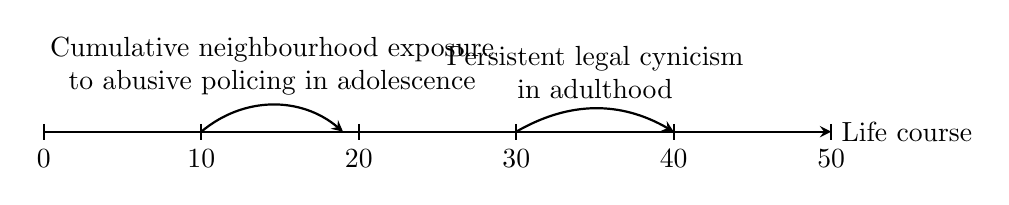
\begin{tikzpicture}[>=stealth, thick]

% Timeline
\draw[->] (0,0) -- (10,0) node[right]{Life course};

% Age ticks
\foreach \x/\lab in {0/0,2/10,4/20,6/30,8/40,10/50}
  \draw (\x,0.1) -- (\x,-0.1) node[below]{\lab};

% Curved arrow: adolescence (10 → 19)
\draw[->, bend left=40] (2,0) to node[above, align=center]
    {Cumulative neighbourhood exposure\\to abusive policing in adolescence} (3.8,0);

% Curved arrow: adulthood (30 → 40)
\draw[->, bend left=30] (6,0) to node[above, align=center]
    {Persistent legal cynicism\\in adulthood} (8,0);

\end{tikzpicture}
\end{document}
